% Created 2020-11-11 Wed 12:14
% Intended LaTeX compiler: pdflatex
\documentclass[11pt]{article}
\usepackage[utf8]{inputenc}
\usepackage[T1]{fontenc}
\usepackage{graphicx}
\usepackage{grffile}
\usepackage{longtable}
\usepackage{wrapfig}
\usepackage{rotating}
\usepackage[normalem]{ulem}
\usepackage{amsmath}
\usepackage{textcomp}
\usepackage{amssymb}
\usepackage{capt-of}
\usepackage{hyperref}
\usepackage{minted}
\author{Ryan \& James}
\date{\today}
\title{The Emergence of Order \begin{center}
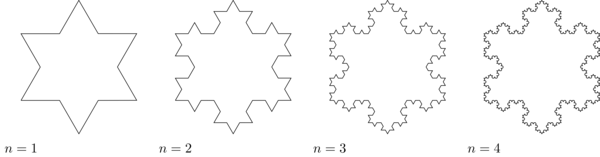
\includegraphics[width=.9\linewidth]{../media/tikz/Snowflake.png}
\end{center}}
\hypersetup{
 pdfauthor={Ryan \& James},
 pdftitle={The Emergence of Order \begin{center}
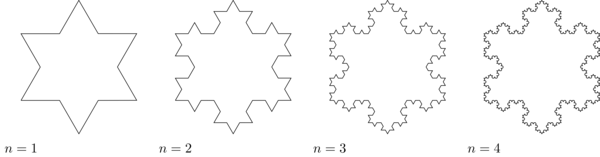
\includegraphics[width=.9\linewidth]{../media/tikz/Snowflake.png}
\end{center}},
 pdfkeywords={},
 pdfsubject={},
 pdfcreator={Emacs 27.1 (Org mode 9.4)}, 
 pdflang={English}}
\begin{document}

\maketitle

\section{Introduction}
\label{sec:org182cc5b}
\begin{itemize}
\item Looked at the emergence of patterns from natural and iterative processes.
\item This lead to an investigation of fractals mostly
\end{itemize}
\section{Definition of a Fractal}
\label{sec:org71bcd3a}
\begin{itemize}
\item Shapes with a complex structure
\item Tend to exhibit self-similarity
\begin{itemize}
\item Although they may not!
\end{itemize}
\end{itemize}

\subsection{Examples of Fractals}
\label{sec:org79fab3c}
To motivate the concept, here are some fractals we generated in our investigation:

\begin{itemize}
\item Self-Similar Fractals
\end{itemize}

\begin{align*}
\mathbf{B} \leftarrow
   \begin{bmatrix}
       \mathbf{B} & \mathbf{Z} & \mathbf{B} \\
       \mathbf{Z} & \mathbf{B} & \mathbf{Z} \\
       \mathbf{B} & \mathbf{Z} & \mathbf{B} \\
   \end{bmatrix}
\end{align*}

where:

\begin{itemize}
\item \(\mathbf{B}= \left[ 1 \right]\)
\item \(\mathbf{Z}= \left[ 0 \right]\)
\end{itemize}

\url{media/vicsek\_fractal.gif}

\begin{align*}
\mathbf{B} \leftarrow
   \begin{bmatrix}
       \mathbf{B} & \mathbf{B} & \mathbf{B} \\
       \mathbf{B} & \mathbf{Z} & \mathbf{B} \\
       \mathbf{B} & \mathbf{B} & \mathbf{B} \\
   \end{bmatrix}
\end{align*}

\url{media/sierpinski\_carpet.gif}


\begin{itemize}
\item Can also use the Chaos Game
\end{itemize}

\begin{center}
\includesvg[width=.9\linewidth]{media/chaos_game/1}
\end{center}
\begin{center}
\includesvg[width=.9\linewidth]{media/chaos_game/2}
\end{center}
\begin{center}
\includesvg[width=.9\linewidth]{media/chaos_game/3}
\end{center}
\begin{center}
\includesvg[width=.9\linewidth]{media/chaos_game/4}
\end{center}
\begin{center}
\includesvg[width=.9\linewidth]{media/chaos_game/5}
\end{center}
\begin{center}
\includesvg[width=.9\linewidth]{media/chaos_game/6}
\end{center}
\begin{center}
\includesvg[width=.9\linewidth]{media/chaos_game/7}
\end{center}
\begin{center}
\includesvg[width=.9\linewidth]{media/chaos_game/8}
\end{center}
\url{media/sierpinsky\_triangle\_chaos.gif}


\begin{itemize}
\item and sometimes thay just fall out of otherwise simple math:
\end{itemize}

\[
z \leftarrow z^{2} + c
\]

\begin{itemize}
\item What follows is an illustration of all the points that converge to zero for values on the circle:
\end{itemize}

\[
z \leftarrow z^{2} + e^{i \frac{9k}{2}}
\]

\url{media/julia\_sets.gif}

\subsection{Generating Fractals}
\label{sec:org9e964e2}
\begin{itemize}
\item Matrices and Iteration
\item Drawing them
\item Chaos Game
\item Recurrence
\end{itemize}
\subsection{Mandelbrots Definition}
\label{sec:orgd2a1602}
\begin{itemize}
\item Defined it as:
\item Later went back on this
\item Efforts have been made to more clearly define it.
\end{itemize}
\subsection{The Fractal Dimension}
\label{sec:org4c9cd29}
\section{Defining Dimension}
\label{sec:orgde077ff}
\subsection{Hausdorff Measure}
\label{sec:org28bf5ee}
\subsection{Hausdorff Dimension}
\label{sec:org1f37539}
\section{My fractal if I have time}
\label{sec:org6e94962}
\section{Measuring the Dimension of a non-self-similar Fractal}
\label{sec:org09a3a4e}
\end{document}